\documentclass{article}
\usepackage[utf8]{inputenc}
\usepackage{fancyhdr}
\usepackage{graphicx}

\title{\textbf{Debian LTS Survey}}
\author{Utkarsh Gupta \\
    \small (utkarsh@debian.org)}
\date{August 15th 2020}

\addtolength{\oddsidemargin}{-.875in}
\addtolength{\evensidemargin}{-.875in}
\addtolength{\textwidth}{1.75in}

\addtolength{\topmargin}{-.875in}
\addtolength{\textheight}{1.75in}

\begin{document}

\maketitle

\vspace{5mm}
\section{Introduction}

On July 18th, Stretch LTS started, offering two more years of security support to the Debian Stretch release. Stretch LTS is the fourth iteration of LTS, following Squeeze LTS which started in 2014, Wheezy LTS in 2016, and Jessie LTS in 2018. \par

\vspace{3mm}
However, for the first time, we prepared a small survey about our users and contributors, who they are and why they are using LTS. This document compiles the results of that very survey.

\vspace{5mm}
\section{Quick Statistics}

\vspace{3mm}
\begin{itemize}
    \item Number of questions: 14
    \item Survey duration: 2 weeks
    \item Survey start date: July 13th, 2020
    \item Survey end date: July 27th, 2020
    \item Total responses: 1764
    \begin{itemize}
        \item Complete responses: 892
        \item Incomplete responses*: 872
    \end{itemize}
\end{itemize}

\fancypagestyle{plain}{
   \fancyhf{} 
   \fancyfoot[L]{* means that those number of surveyees didn't fill each and every question and
   skipped some of them.}
   \renewcommand{\headrulewidth}{0pt}
   \renewcommand{\footrulewidth}{0.5pt}
}

\vspace{3mm}
\section{Responses}

\vspace{3mm}
We've got an overwhelming response from the survey. Below are the responses and the stats.

\newpage

\begin{figure}
\centering
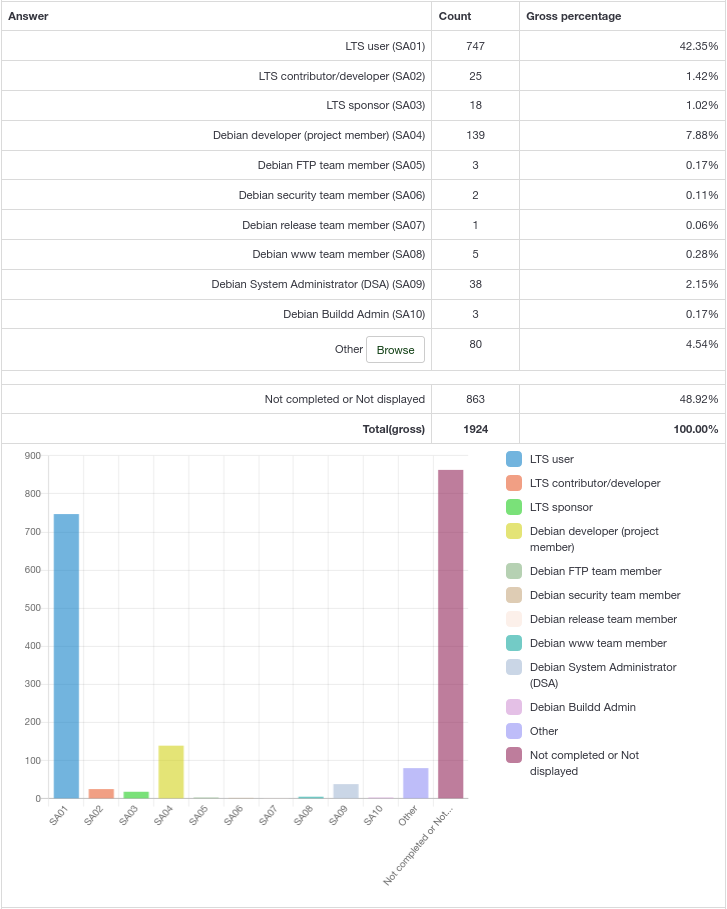
\includegraphics[width=15cm]{assets/1-summary.png}
\caption{Summary of Response 1}
\end{figure}

\end{document}
